% \documentclass{article}
\documentclass[tikz,margin=5mm]{standalone}
\usepackage{tikz}
\begin{document}
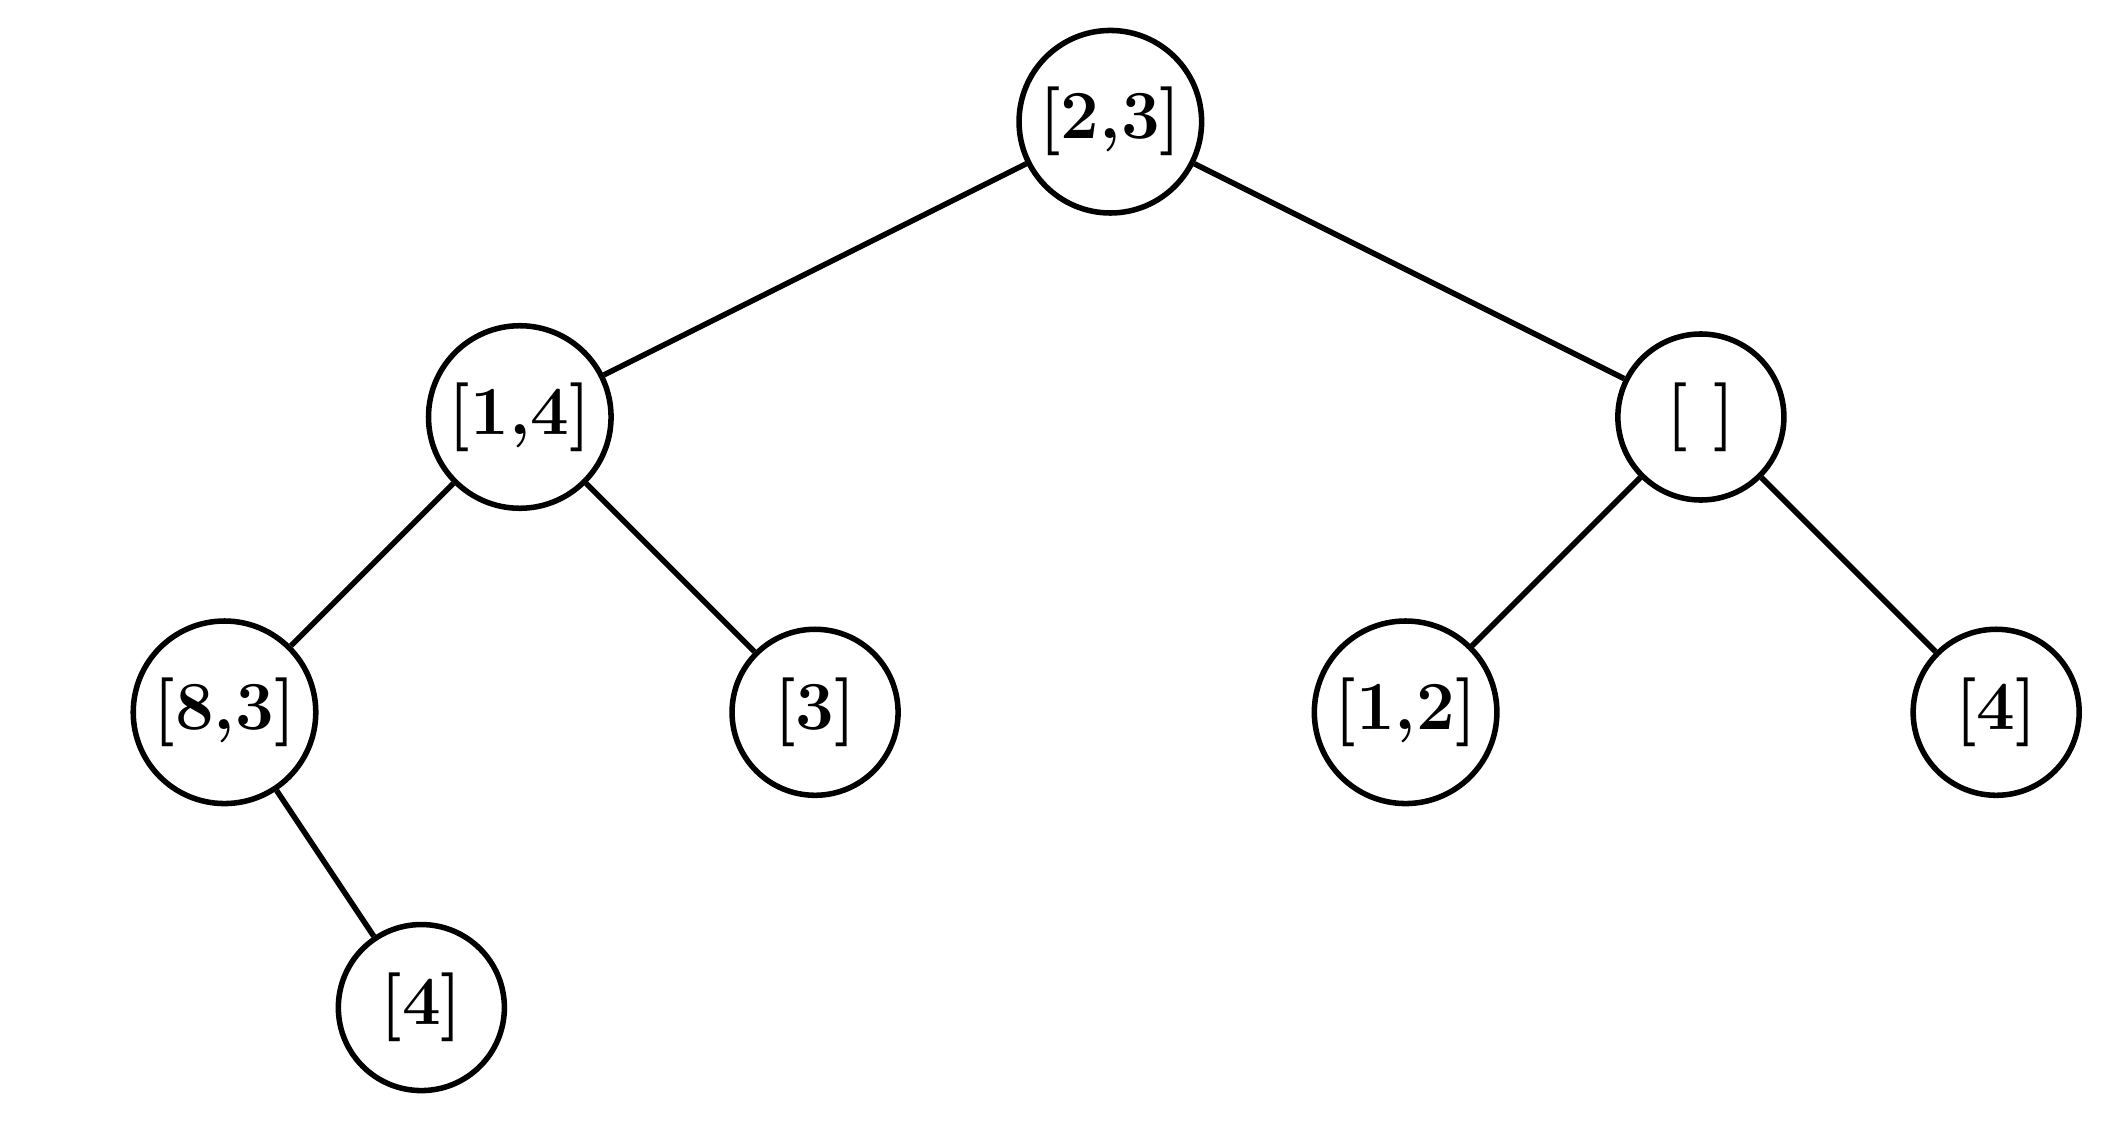
\begin{tikzpicture}[
  scale=2.5,
  every node/.style = {minimum width = 6em, draw, circle, font=\Huge\bf, line width=2pt, scale=1},
  edge from parent/.style={line width=2pt, draw},
  level/.style = {sibling distance = 60mm/#1}
]
\node {[2,3]}
  child {
    node {[1,4]}  
        child {
          node {[8,3]}
          child {edge from parent[draw = none]}
          child {node {[4]}}
        }
        child {
          node {[3]}
          % child {node {I}}
          % child {edge from parent[draw = none]}
        }
      }
  child {
    node {[ ]}
    child {
      node {[1,2]}
    }
    child {
      node {[4]}
      % child {edge from parent[draw = none]}
      % child {node{M}}
    }
    };
\end{tikzpicture}
\end{document}

